\documentclass[a4paper]{article}

\usepackage{tecnico_relatorio}

\usepackage{textcomp}
\usepackage[hypcap]{caption} % makes \ref point to top of figures and tables
%\usepackage{rotating}
\usepackage{float}
\usepackage[nottoc]{tocbibind}
\usepackage[utf8]{inputenc}
\usepackage{graphicx}
\usepackage[justification=centering]{caption}
\usepackage{listings}
\usepackage{indentfirst} % indent first paragraph in section

\begin{document}
	\trSetImage{img/tecnico_logo}{6cm} % Logotipo do Técnico
    
    \trSetCourse{Mestrado em Engenharia Electrotécnica \\e de Computadores}
    
	\trSetSubject{Programação Orientada por Objectos}
	%\trSetType{Projecto}
	\trSetTitle{Aprendizagem de Redes de Bayes Dinâmicas}

	\trSetBoxStyle{0.3}

	\trSetGroupNo{Grupo 22}

	\trSetAuthorNr{2}

	\trSetAuthors
	{
		\begin{center}
			Gonçalo Ribeiro

			73294
		\end{center}
	}{
		\begin{center}
			Francisco Leal

			72939
		\end{center}
	}

	\trSetProfessor{Prof. Alexandra Carvalho}

	\trMakeCover

	\tableofcontents
	\pagenumbering{gobble}

	\pagebreak

	\pagenumbering{arabic}
	\setcounter{page}{1}


	


	\section{Objectivos}

	O objectivo deste projecto consiste em utilizar uma rede de Bayes dinâmica (DBN) para modelar uma \textit{multivariate time series} (MTS). São usados dados para treinar uma rede de Bayes e de seguir são previstos valores a partir de um conjunto de dados de teste e da rede treinada.
    
    A implementação utiliza os conceitos aprendidos nas aulas de Programação Orientada por Objectos tanto quanto possível, de forma a que a implementação possa ser extensível.
	


	\section{Algoritmos}

      \subsection{\textit{Greedy Hill Climbing} -- GHC}

      Para treinar utilizou-se o algoritmo \textit{greedy hill climbing} (GHC). Este algoritmo ``experimenta'' os vizinhos da rede actual, calcula o \textit{score} desses vizinhos e tenta avançar para uma rede com um \textit{score} melhor do que aquele atingido até ao momento.
      
      O GHC tem variantes: na sua versão mais simples o algoritmo para logo que não consegue encontrar uma rede vizinha com \textit{score} melhor que a \textit{score} actual. Isto permite apenas chegar a máximos locais. Numa segunda abordagem quando se atinge um máximo local faz-se uma reinicialização das arestas da rede e recomeça-se o GHC simples até que se atinja novo máximo local. Fazendo várias iterações espera-se atingir um máximo local que coincida com o global. Uma última abordagem usa \textit{tabu search}, o que significa que é guardado um histórico das últimas configurações que foram tentadas e que essas configurações não voltam a ser visitadas.
      
      Foi implementado o GHC simples e o GHC com \textit{random restarts}. A implementação com \textit{tabu} foi pensada e iniciada mas não foi concluída por limitações temporais.

      \subsection{Verificação de Grafo Acíclico}
      
      Ao fazer as operações elementares de adicionar, inverter e remover arestas da \textit{transition network} temos sempre que garantir que a rede é acíclica. Com este objectivo concebeu-se um algoritmo baseado no algoritmo de Tarjan que nos permite saber se um grafo é acíclico ou não.
      
      O algoritmo de Tarjan serve para encontrar componentes fortemente conexas de um grafo. Num grafo acíclico o número de componentes fortemente conexas coincide com o número de nós. No entanto para resolver o problema de se um grafo é acíclico não é preciso determinar as componentes fortemente conexas, ou seja é possível usar um algoritmo mais simples do que o de Tarjan. O algoritmo implementado utiliza dois marcadores por cada nó: um marcador que indica se o nó foi visitado e outro que marca se o nó está no caminho correntemente a ser explorador ou não. O algoritmo percorre o grafo com uma DFS (\textit{depth first search} e vai marcando os nós como visitados. Marca também os nós que estão no caminho actual desde o nó em que se começou a DFS. Se for encontrado um nó que já está visitado e que está no caminho actual então isso significa que é formado um ciclo através desse nó, pelo que o grafo não é acíclico.
      
      Visto que o grafo pode não ser conexo pode ser preciso correr o algoritmo para todas as componentes conexas do grafo. No pior caso---que é o grafo ser acíclico ou o ciclo só ser encontrado após visitar todos os nós---é preciso marcar todos os nós como visitados e são visitadas todas as arestas pelo que a complexidade do algoritmo é $O(n+m)$ em que $n$ é o número de nós do grafo e $m$ é o número de arestas.



      \section{Estruturas de Dados}
	  Existem duas estruturas de dados criadas pelo grupo, \textit{Slice} e \textit{Data}.
      
      \textit{Data} é utilizado de modo a traduzir o conteúdo dos ficheiros \texttt{\.csv} para dados, do tipo \texttt{int}. De modo a resolver o problema dos dados poderem não ser rectangulares, quando existem linhas de dados incompletas esses são substituídos pelo marcador \texttt{-1}.
      
      \textit{Slice} é utilizado para realizar a divisão da Data em \textit{time slices}. Cada \textit{slice} representa um instante de tempo distinto, tornando mais fácil aceder a um tempo específico noutras partes da aplicação.
      
      As outras estruturas de dados que são utilizadas e que fazem parte das estruturas do Java são \texttt{HashSet} e \texttt{ArrayList}. \texttt{HashSet} é usada para guardar os vizinhos de cada nó e foi escolhida pelo facto de ser necessário muitas vezes fazer procuras para saber se um elemento já está presente na lista de arestas de um nó. A complexidade da procura num \texttt{HashSet} é de $0(1)$ (em média) enquanto que na maioria das outras estruturas esta procura seria O(n). De facto e média também a inserção e remoção são $O(1)$ para um \texttt{HashSet}.
      \textit{ArrayList} foi escolhido por permitir ser um vector dinâmico e ter complexidade de acesso e de inserção de $O(1)$. Foi utilizado onde estas propriedades se justificassem.

	  Para a realização da \texttt{TabuList} foi decidido utilizar um \texttt{HashSet} devido às suas propriedades de complexidade já descritas. Neste \texttt{HashSet} guardamos os \texttt{hashCodes} das estruturas por onde já se passou. Esta implementação é possível devido ao baixo número de estruturas testadas durante o algoritmo GHC, que faz com que não deva existir um número significativo de colisões entre os \texttt{hashCodes} de modo a justificar utilizar outra forma de saber se uma dada estrutura de grafo já foi visitada. Com esta solução há a possibilidade de, devido a uma colisão, não visitarmos uma estrutura que não foi de facto ainda visitada. No entanto consideramos que o número de vezes que isto acontece é desprezável.
      
      
	\begin{figure}[h]
    	\centering
		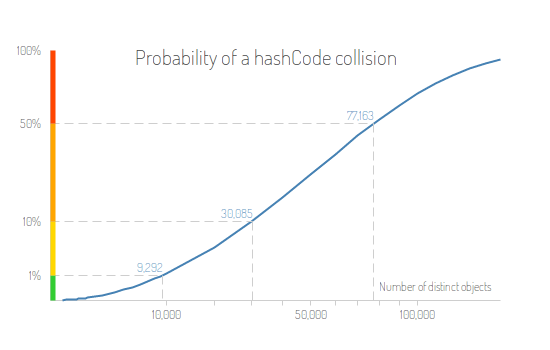
\includegraphics[width=.8\textwidth]{img/hashcode-collisions.png}
        \caption{Probabilidade de colisão em função do número de objectos}
        \label{fig:hashset_colisions}
	\end{figure}



	\section{Ingredientes de POO}

	Durante a elaboração de todo o Projecto, sempre que possível e fosse justificável tentou-se que a forma como cada classe implementa os seus métodos apenas influenciasse a classe em si e nunca as classes que a utilizam. Da mesma maneira também se tentou que o código fosse o mais reaproveitável possível, sendo que qualquer utilizador pode implementar o seu próprio método de treinar a estrutura da rede de Bayes, o seu próprio método de \textit{score} para avaliar se a estrutura alcançada é uma boa estrutura ou não e um método para avaliar se uma rede é um grafo acíclico. Os métodos que foram implementados neste projecto têm tendência a favorecer estruturas completas em vez de estruturas menos ligadas, pelo que pode ter interesse para um programador implementar um novo método de \textit{scoring} e utilizá-lo de uma forma \textit{plug and play} com o resto da aplicação.


	\section{GUI}
    
    Começou-se uma implementação de uma GUI. Nela é possível seleccionar o ficheiro que se pretende usar para treinar a rede e o ficheiro a partir do qual se pretende inferir valores. A interface pede também os parâmetros necessários à execução do programa, como o número de \textit{random restarts} e a \textit{score} a usar durante o treino da rede.
    
    No entanto por falta de tempo a GUI não se pôs a funcionar em conjunto com o resto do programa, pelo que se encontra num \texttt{main()} à parte em que dá para verificar o que foi feito.
    


	\section{Conclusão}
	
    Após a implementação e teste das diferentes implementações do GHC, foi possível verificar que apesar do GHC para algumas situações ser capaz de alcançar o valor máximo da estrutura global, na maioria dos casos isto não acontece, enquanto que ao implementar GHC com \textit{random restarts} começa a ser mais frequente chegar ao máximo global, desde que se use um valor alto o suficiente para que o número de \textit{random restarts} permita testar algumas estruturas diferentes. Apesar de não ter sido possível testar o GHC com \textit{tabu list}  e \textit{random restarts}, durante os vários testes efectuados para a elaboração do projecto, verificou-se que efectivamente existiam muitas estruturas que eram visitadas mais do que uma vez, pelo que a utilização de \textit{tabu} ajudaria a alcançar mais rapidamente e com maior grau de fidelidade o valor máximo global para os dados de treino.








\end{document}